\chapter{Architectures Directed Acyclic Graphs}
We will report here the details of the Directed Acyclic Graphs (DAGs) describing the computational graphs of each of the ANNs architectures used in this thesis. The graphs are generated by the Keras library plotting functionality \cite{chollet2015keras}.

\section{Dynamic Prediction of Future Behavioural Intensity}
The DAGs presented in this section refers to the architectures used in the second iteration of the model building  presented in section \ref{model_architecture_2}. 

\subsection{ENet Architecture}
\begin{figure}[H]
\centering
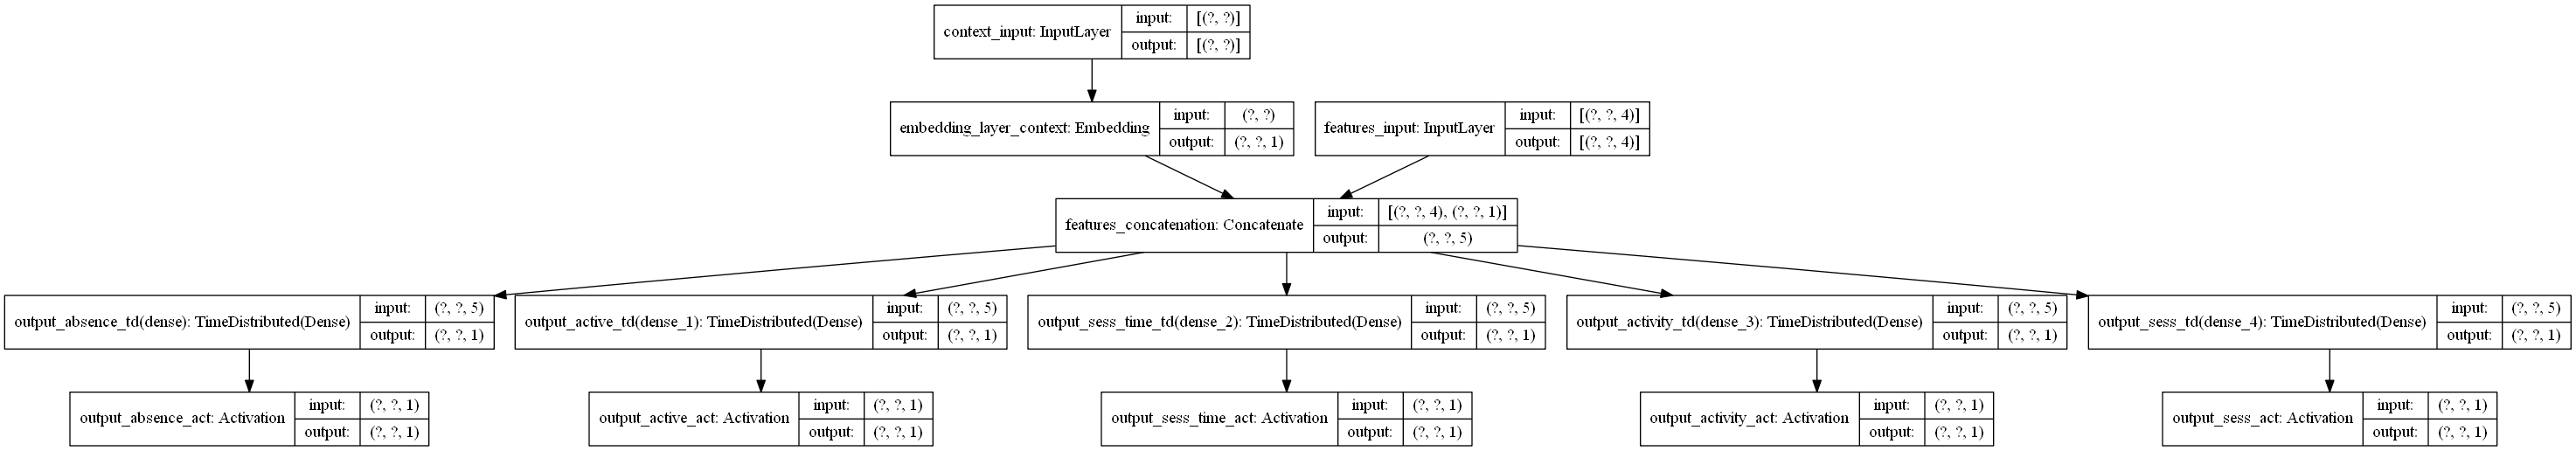
\includegraphics[width=\textwidth,height=\textheight,keepaspectratio]{images/appendix_B/enet_2.png}
\caption[\textbf{ElasticNet DAG - Section \ref{model_architecture_2}}]{Directed acyclic graph representation of the ElasticNet architecture used as a comparison in section \ref{model_architecture_2}}
\label{enet_2_dag}
\end{figure}

\subsection{MLP Architecture}

\begin{figure}[H]
\centering
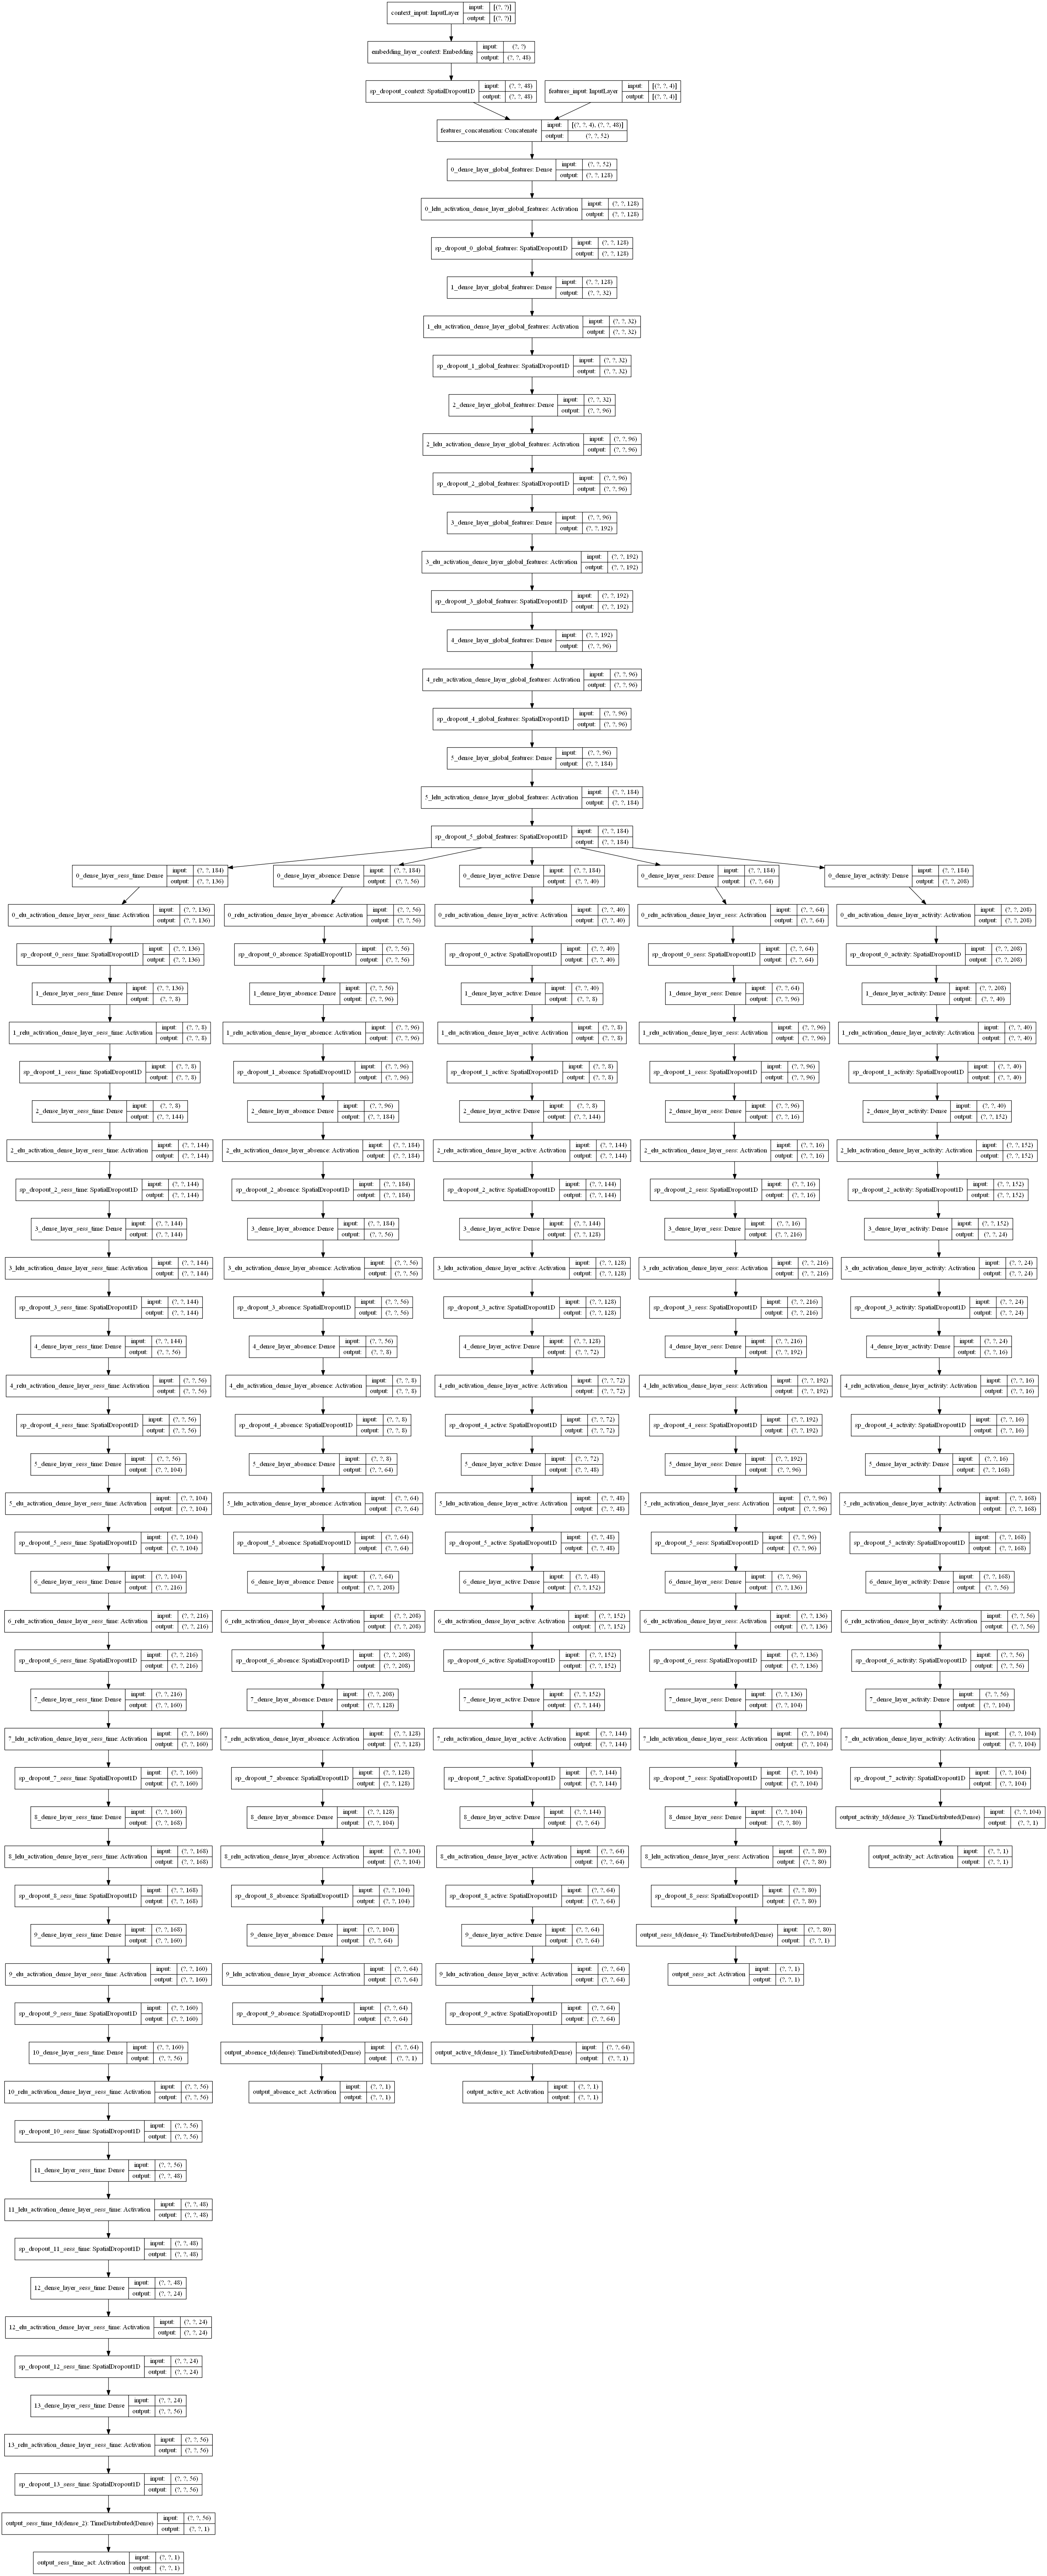
\includegraphics[width=\textwidth,height=0.7\textheight,keepaspectratio]{images/appendix_B/mlp_2.png}
\caption[\textbf{MLP DAG - Section \ref{model_architecture_2}}]{Directed acyclic graph representation of the MLP architecture used as a comparison in section \ref{model_architecture_2}}
\label{mlp_2_dag}
\end{figure}

\subsection{RNN Architecture}

\begin{figure}[H]
\centering
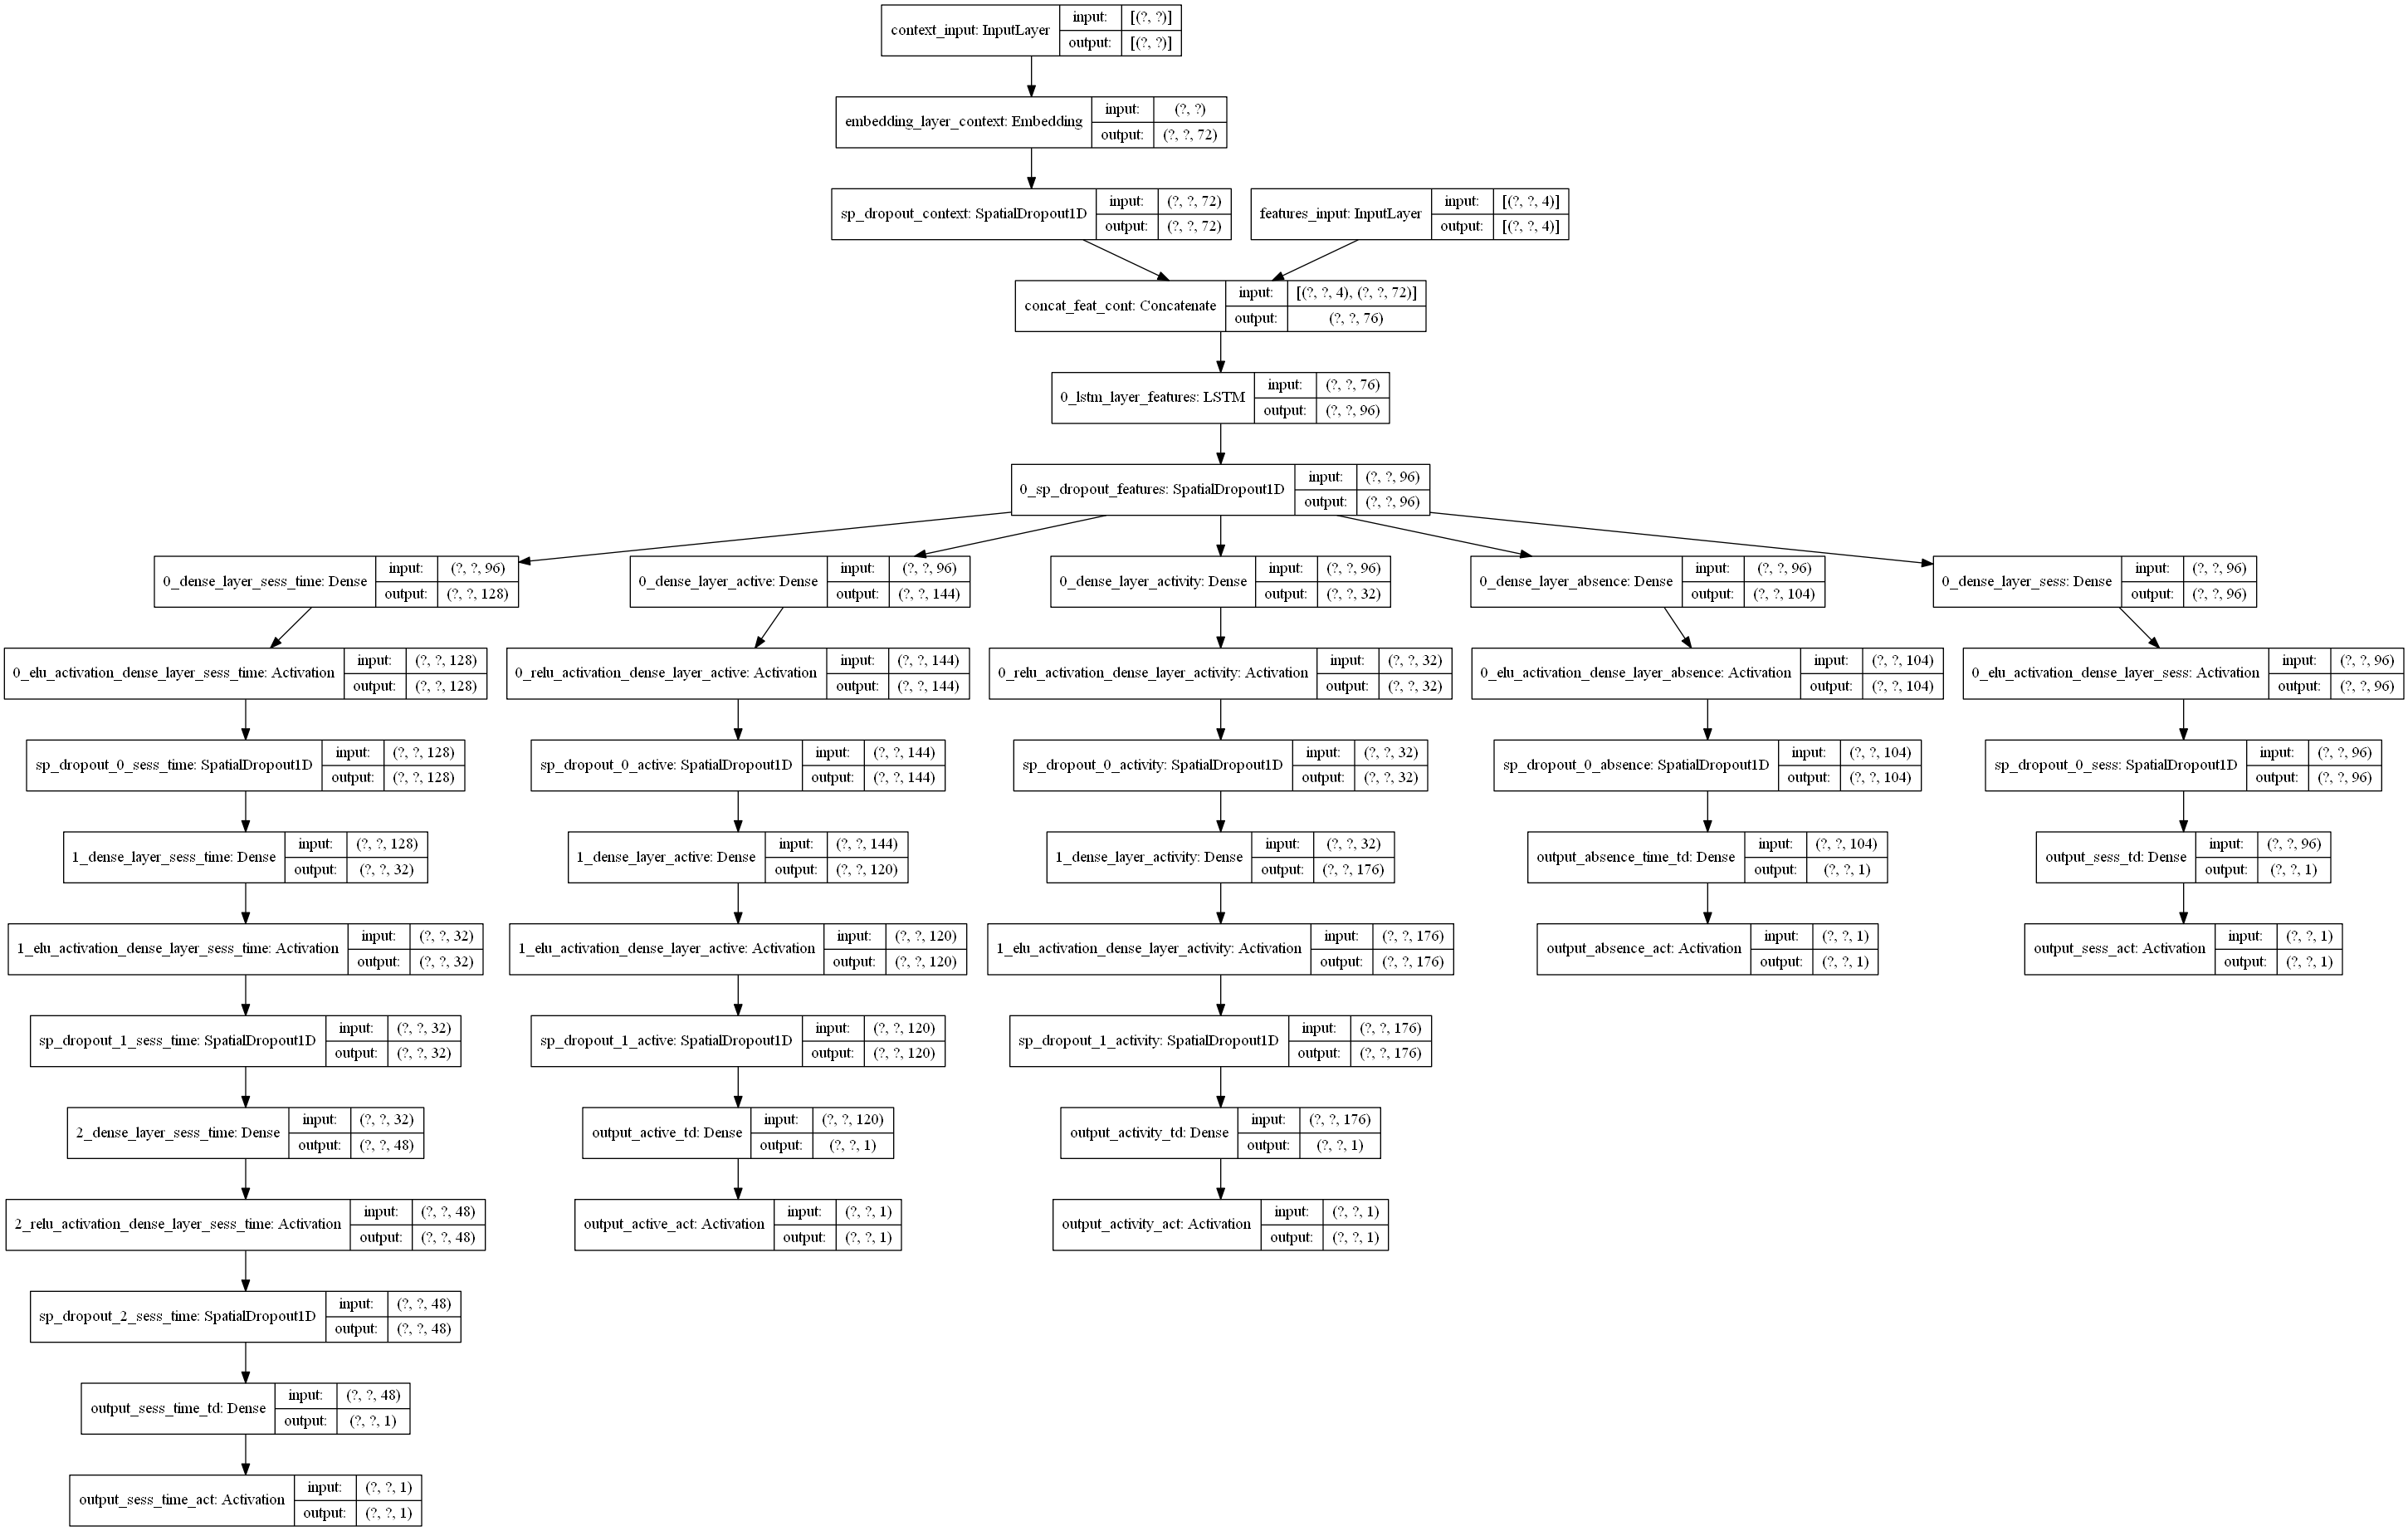
\includegraphics[width=\textwidth,height=\textheight,keepaspectratio]{images/appendix_B/rnn_2.png}
\caption[\textbf{RNN DAG  - Section \ref{model_architecture_2}}]{Directed acyclic graph representation of the RNN architecture proposed in section \ref{model_architecture_2}}
\label{rnn_2_dag}
\end{figure}

\section{Dynamic Prediction of Future Behavioural Intensity with Environmental and Game Covariates}
The DAGs presented in this section refers to the architectures used in the third and last iteration of the model building  presented in section \ref{model_architecture_3}. 

\subsection{MLP Architecture}
\begin{figure}[H]
\centering
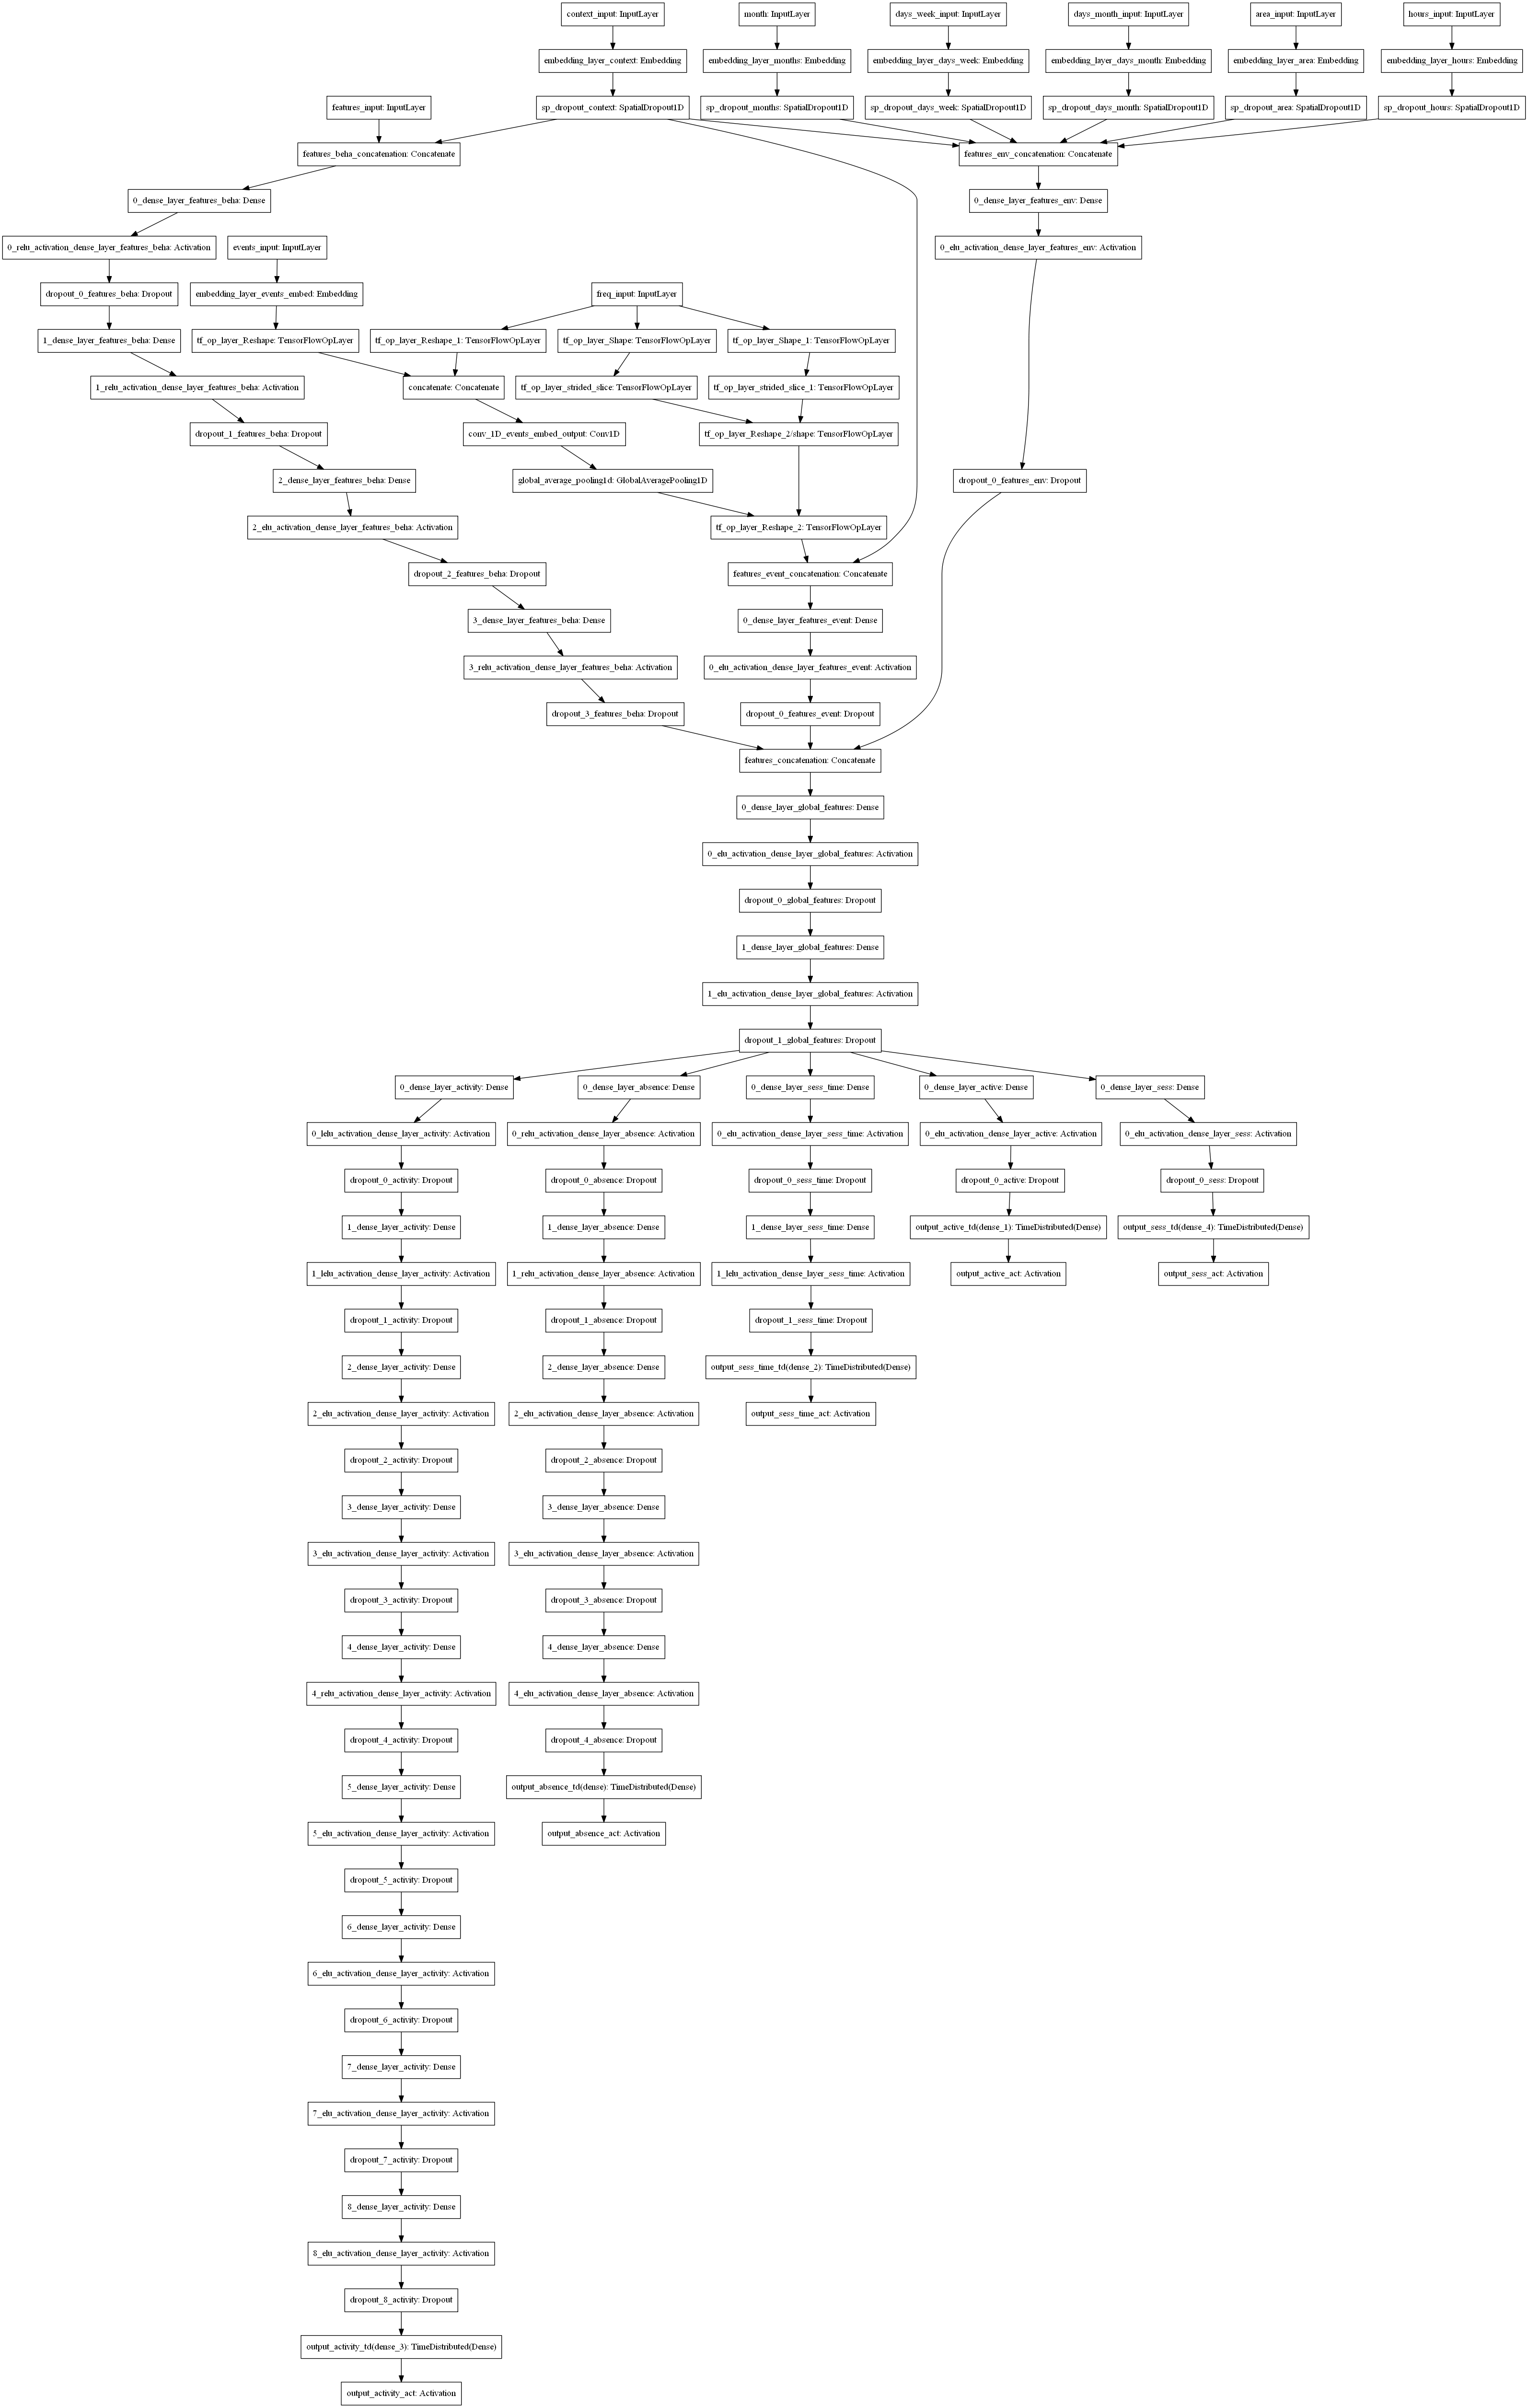
\includegraphics[width=\textwidth,height=0.7\textheight,keepaspectratio]{images/appendix_B/mlp_3.png}
\caption[\textbf{MLP DAG - Section \ref{model_architecture_3}}]{Directed acyclic graph representation of the MLP architecture used as a comparison in section \ref{model_architecture_3}}
\label{mlp_3_dag}
\end{figure}


\subsection{RNN Architecture}
\begin{figure}[H]
\centering
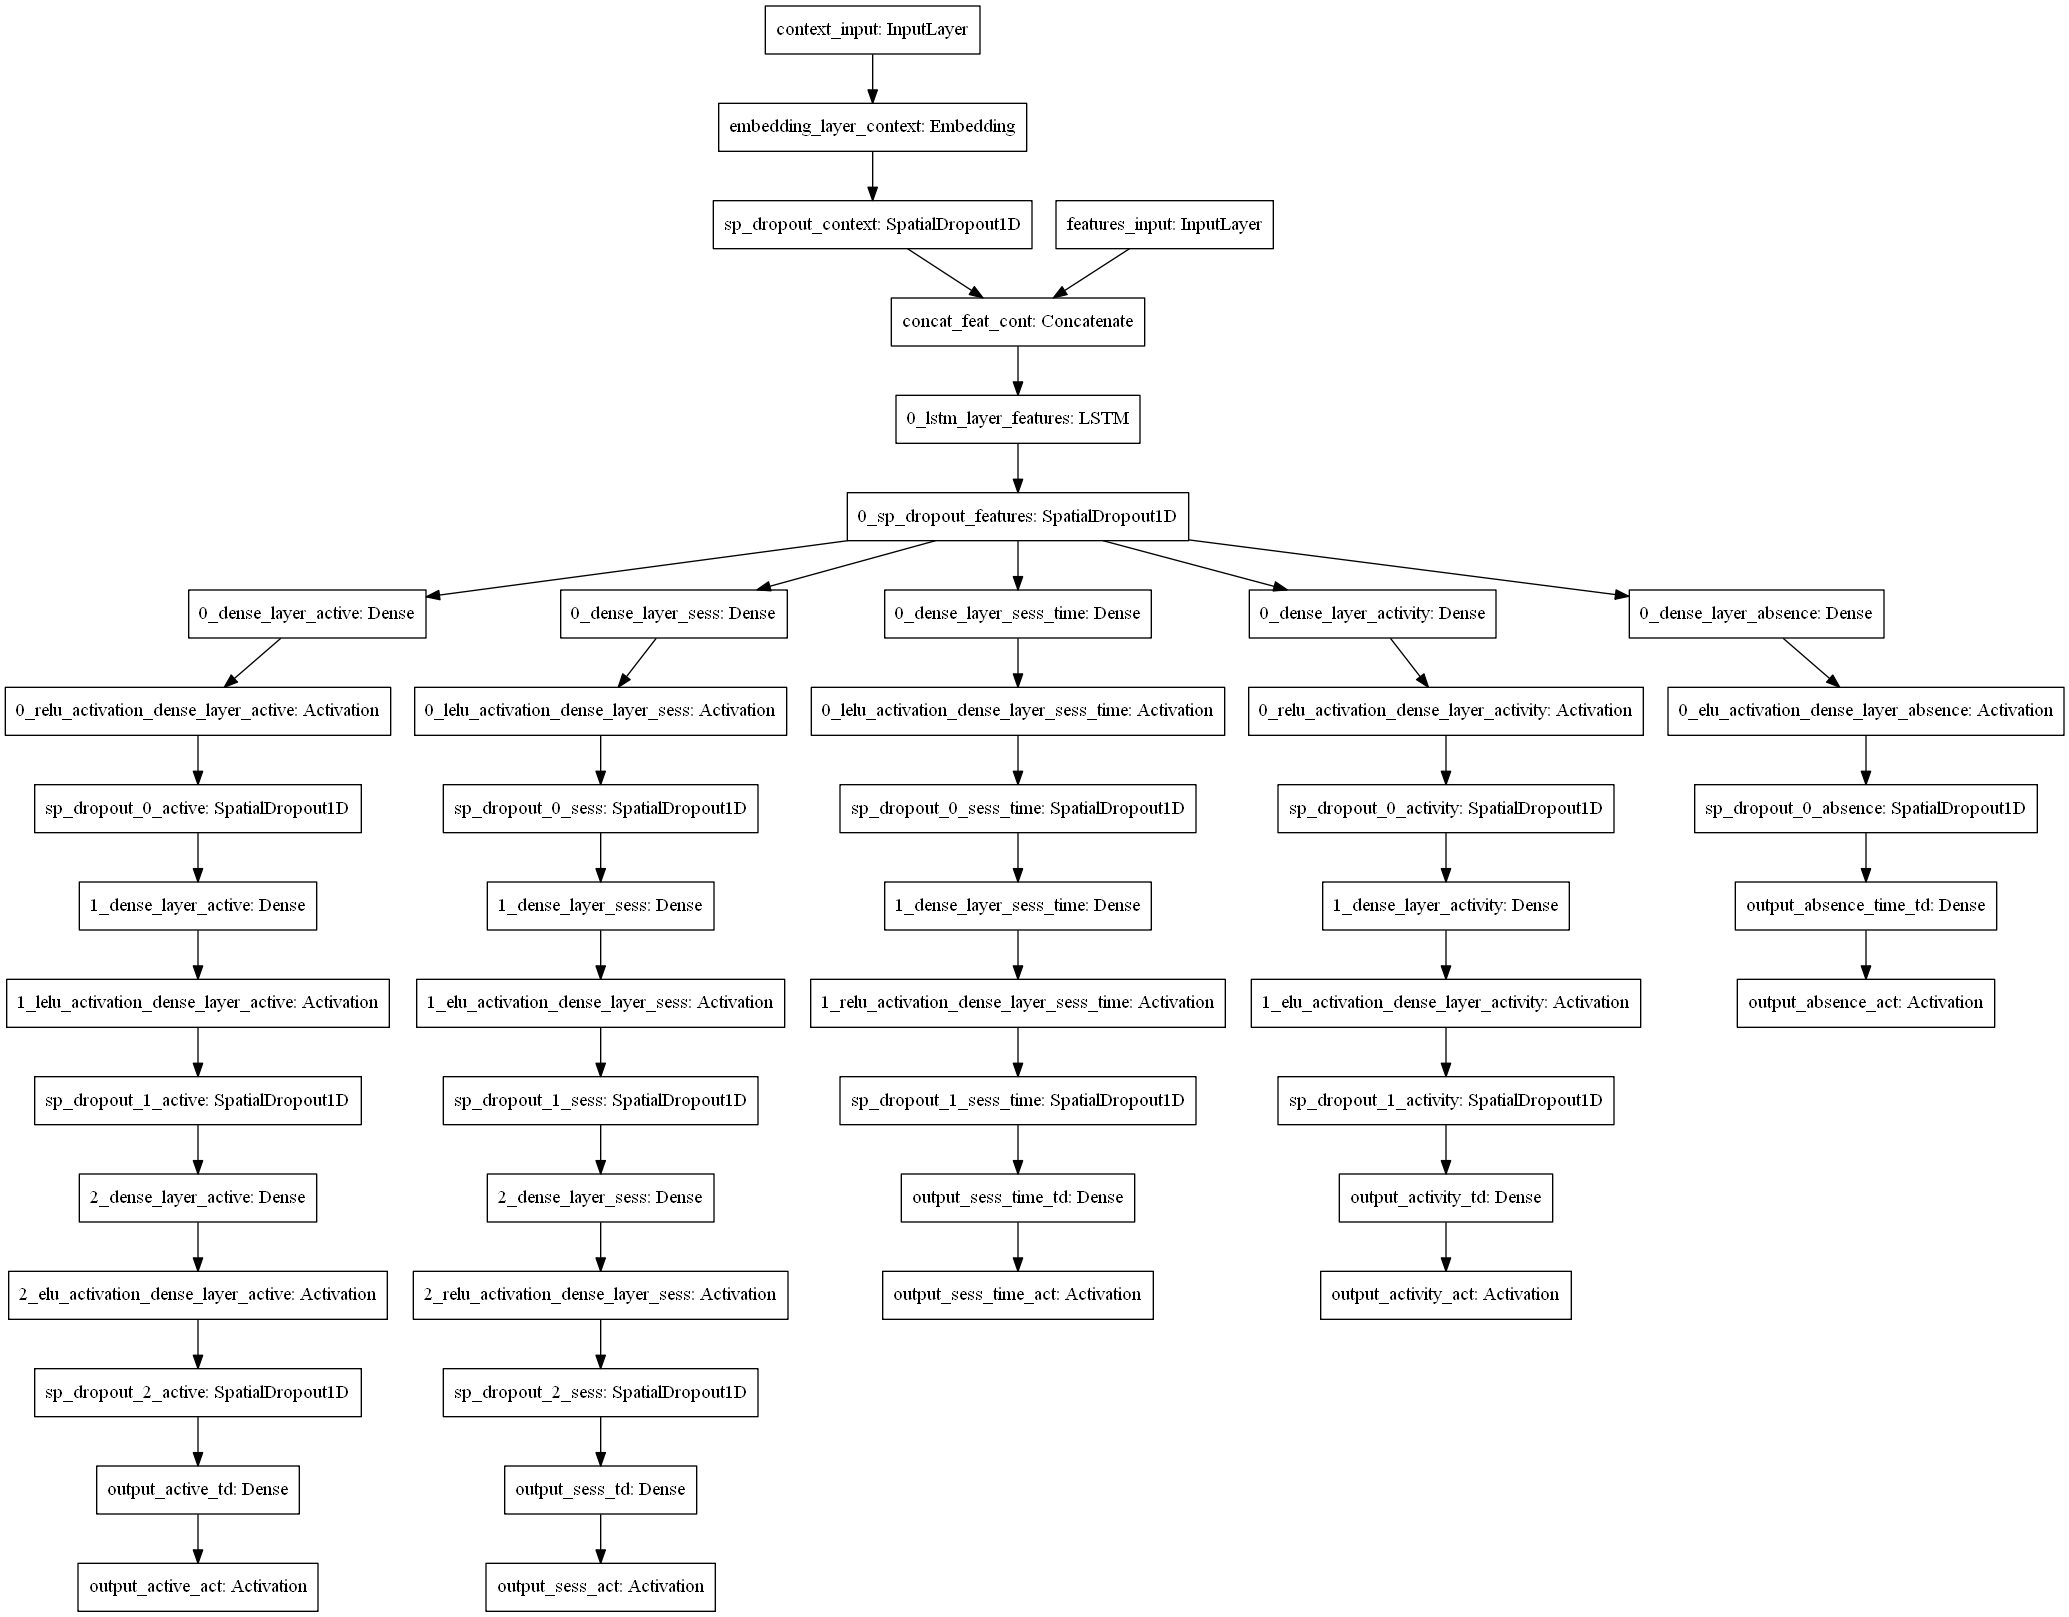
\includegraphics[width=\textwidth,height=0.7\textheight,keepaspectratio]{images/appendix_B/rnn_3.png}
\caption[\textbf{RNN DAG - Section \ref{model_architecture_3}}]{Directed acyclic graph representation of the RNN architecture used as a comparison in section \ref{model_architecture_3}}
\label{rnn_3_dag}
\end{figure}

\subsection{RNN Environment Architecture}
\begin{figure}[H]
\centering
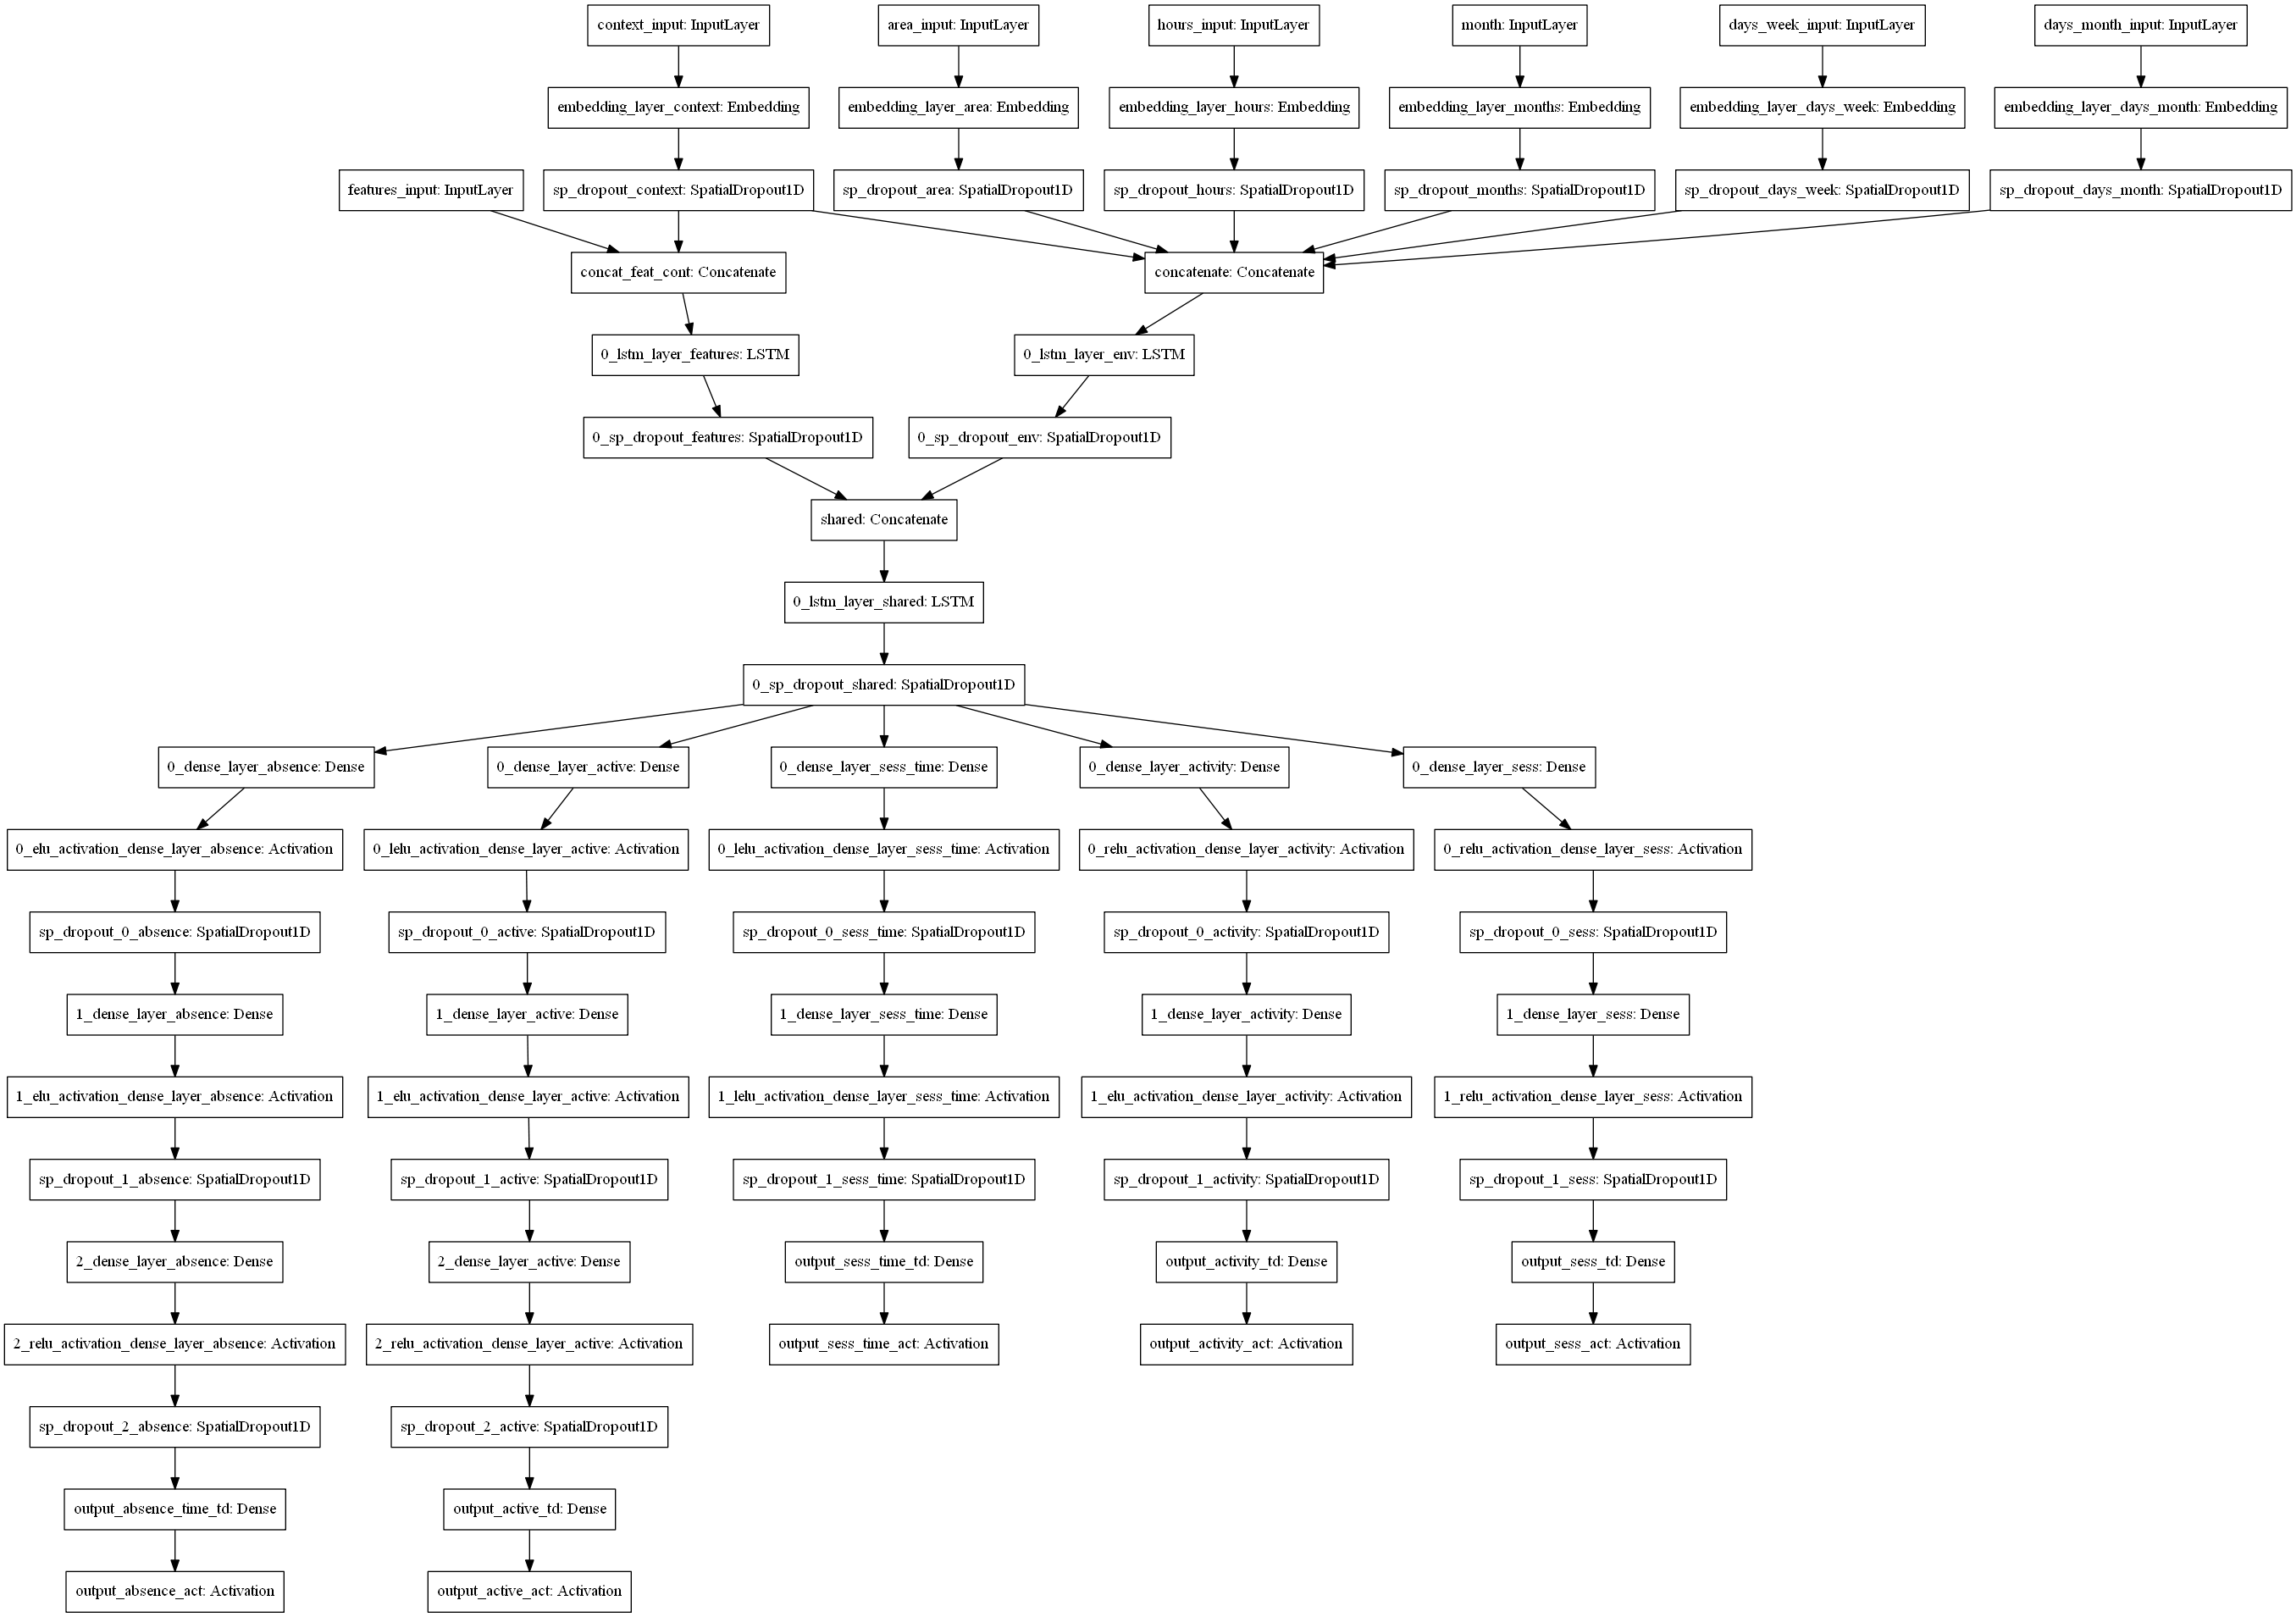
\includegraphics[width=\textwidth,height=0.7\textheight,keepaspectratio]{images/appendix_B/rnn_env_3.png}
\caption[\textbf{RNN Environment DAG - Section \ref{model_architecture_3}}]{Directed acyclic graph representation of the RNN Environment architecture used as a comparison in section \ref{model_architecture_3}}
\label{rnn_env_dag}
\end{figure}

\subsection{RNN Events Architecture}
\begin{figure}[H]
\centering
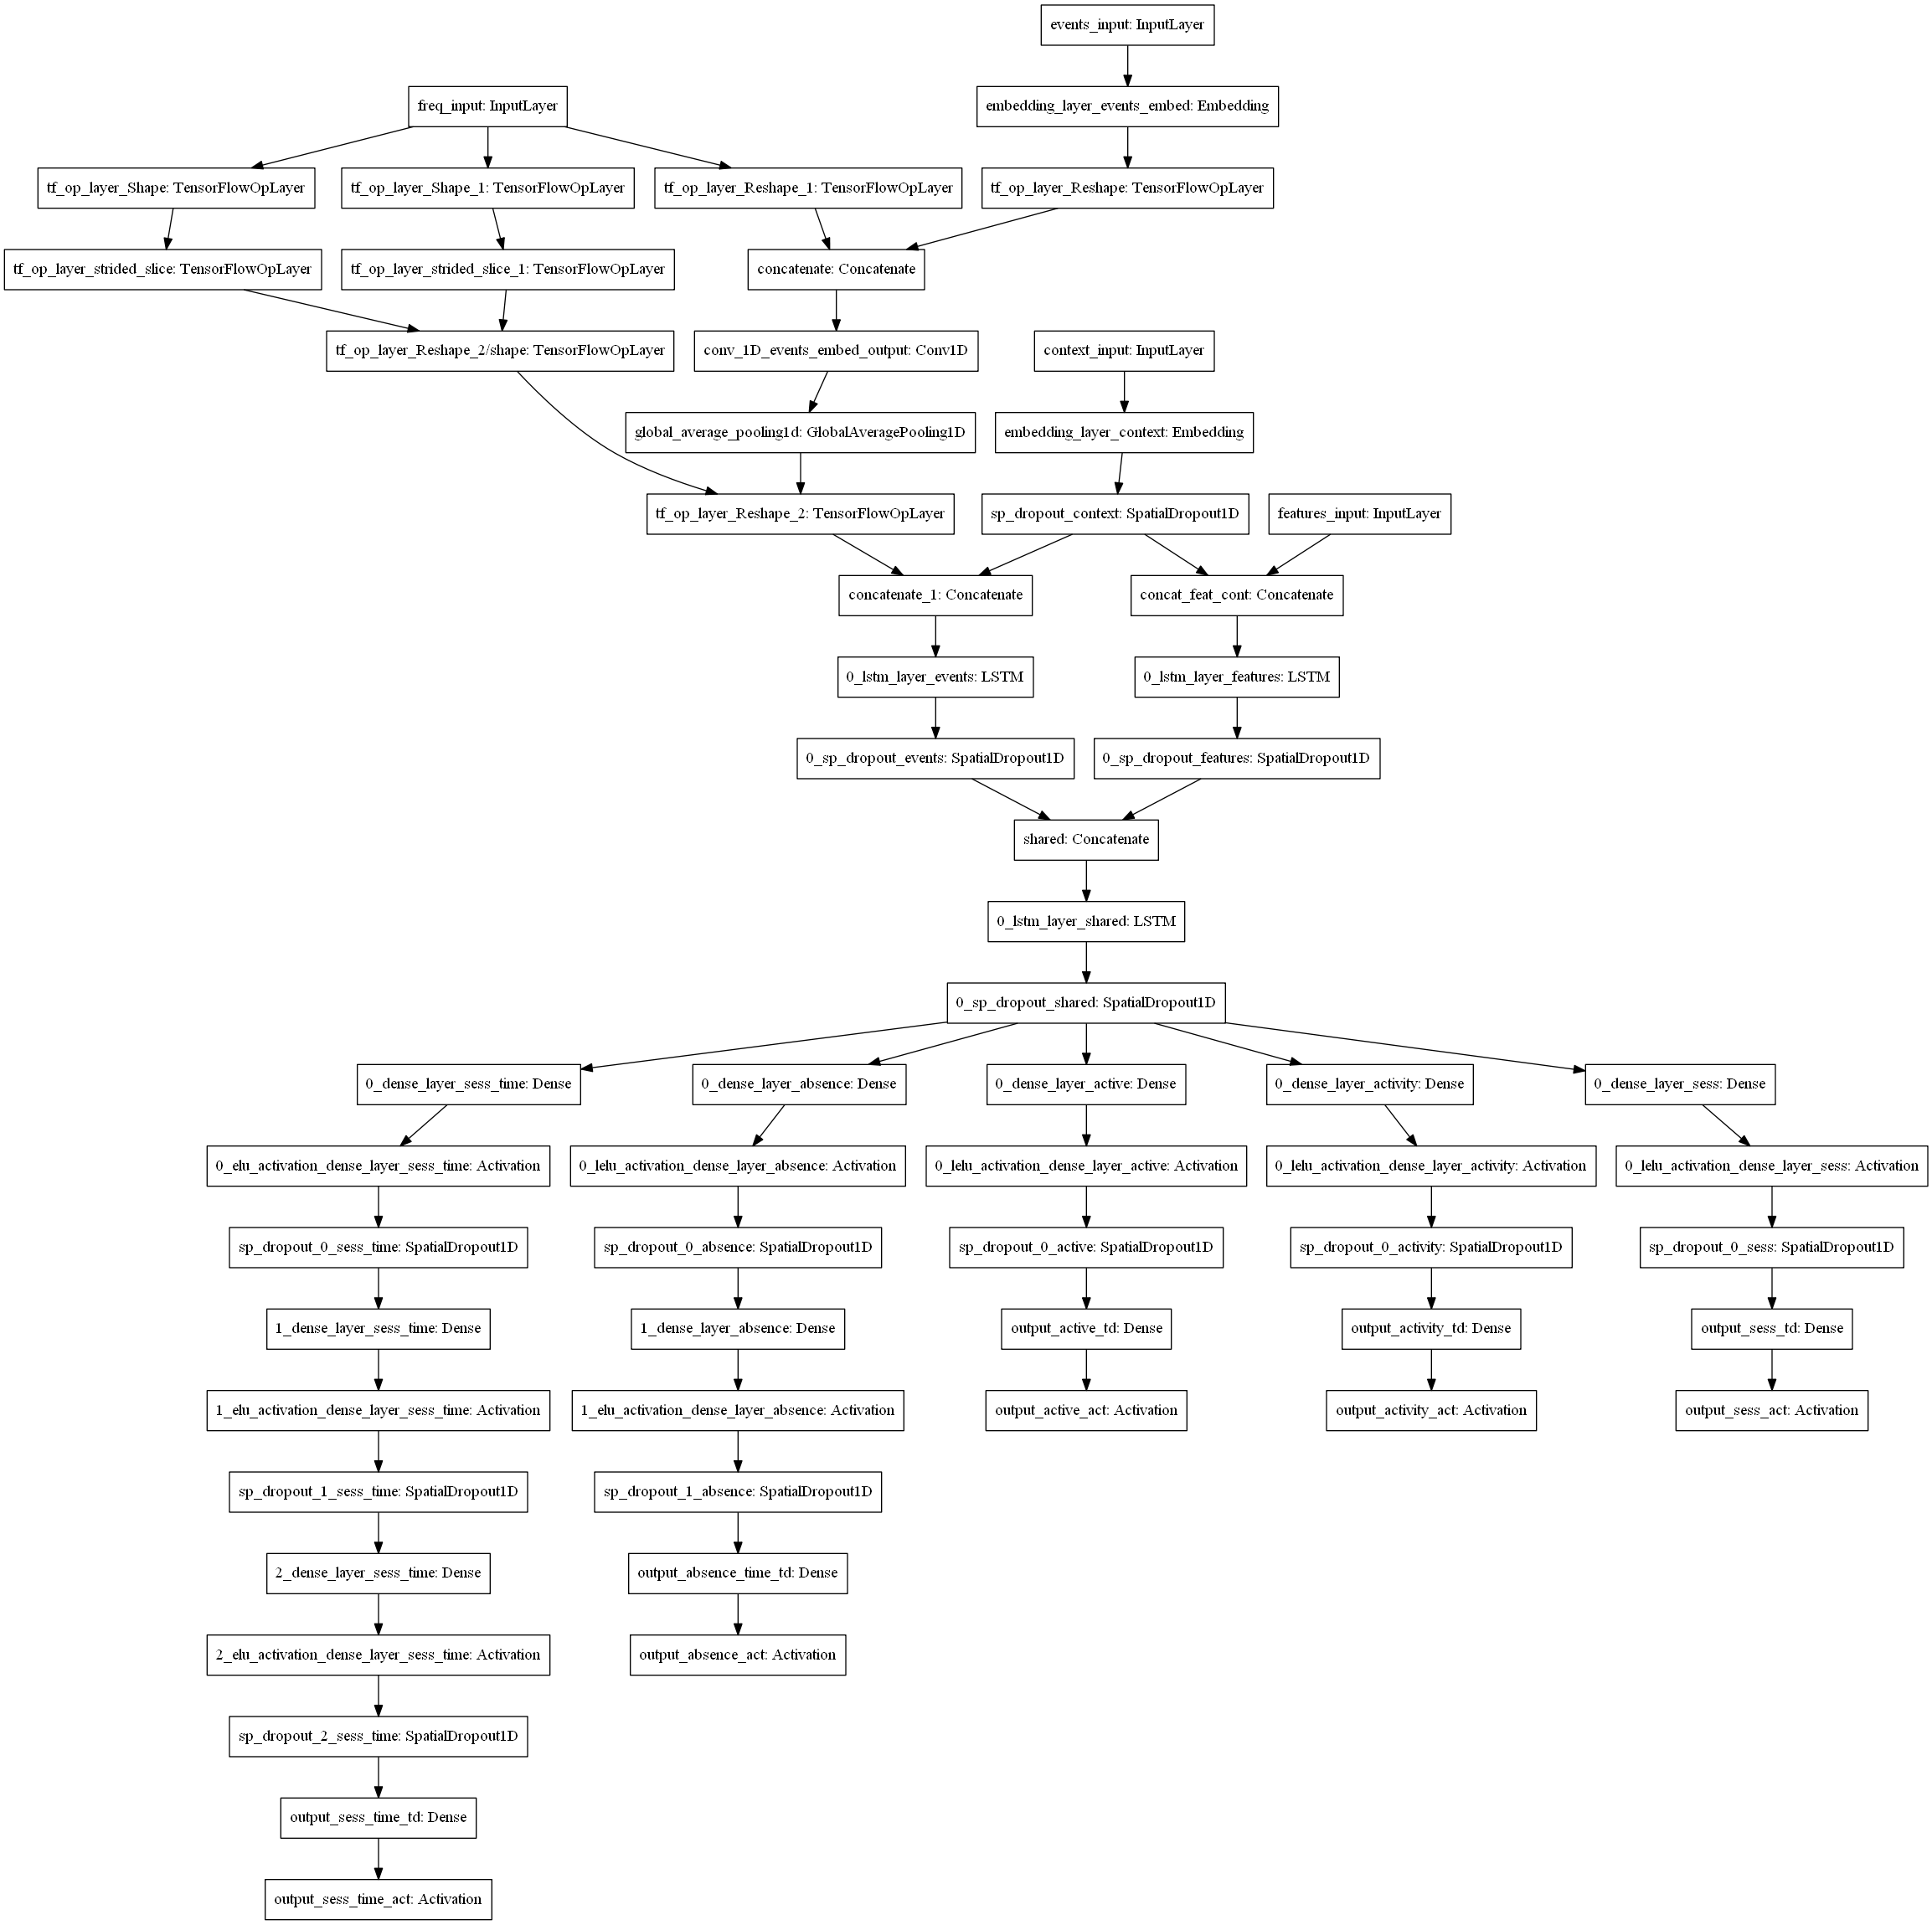
\includegraphics[width=\textwidth,height=0.7\textheight,keepaspectratio]{images/appendix_B/rnn_even_3.png}
\caption[\textbf{RNN Events DAG - Section \ref{model_architecture_3}}]{Directed acyclic graph representation of the RNN Events architecture used as a comparison in section \ref{model_architecture_3}}
\label{rnn_even_dag}
\end{figure}

\subsection{RNN Environment-Events Architecture}
\begin{figure}[H]
\centering
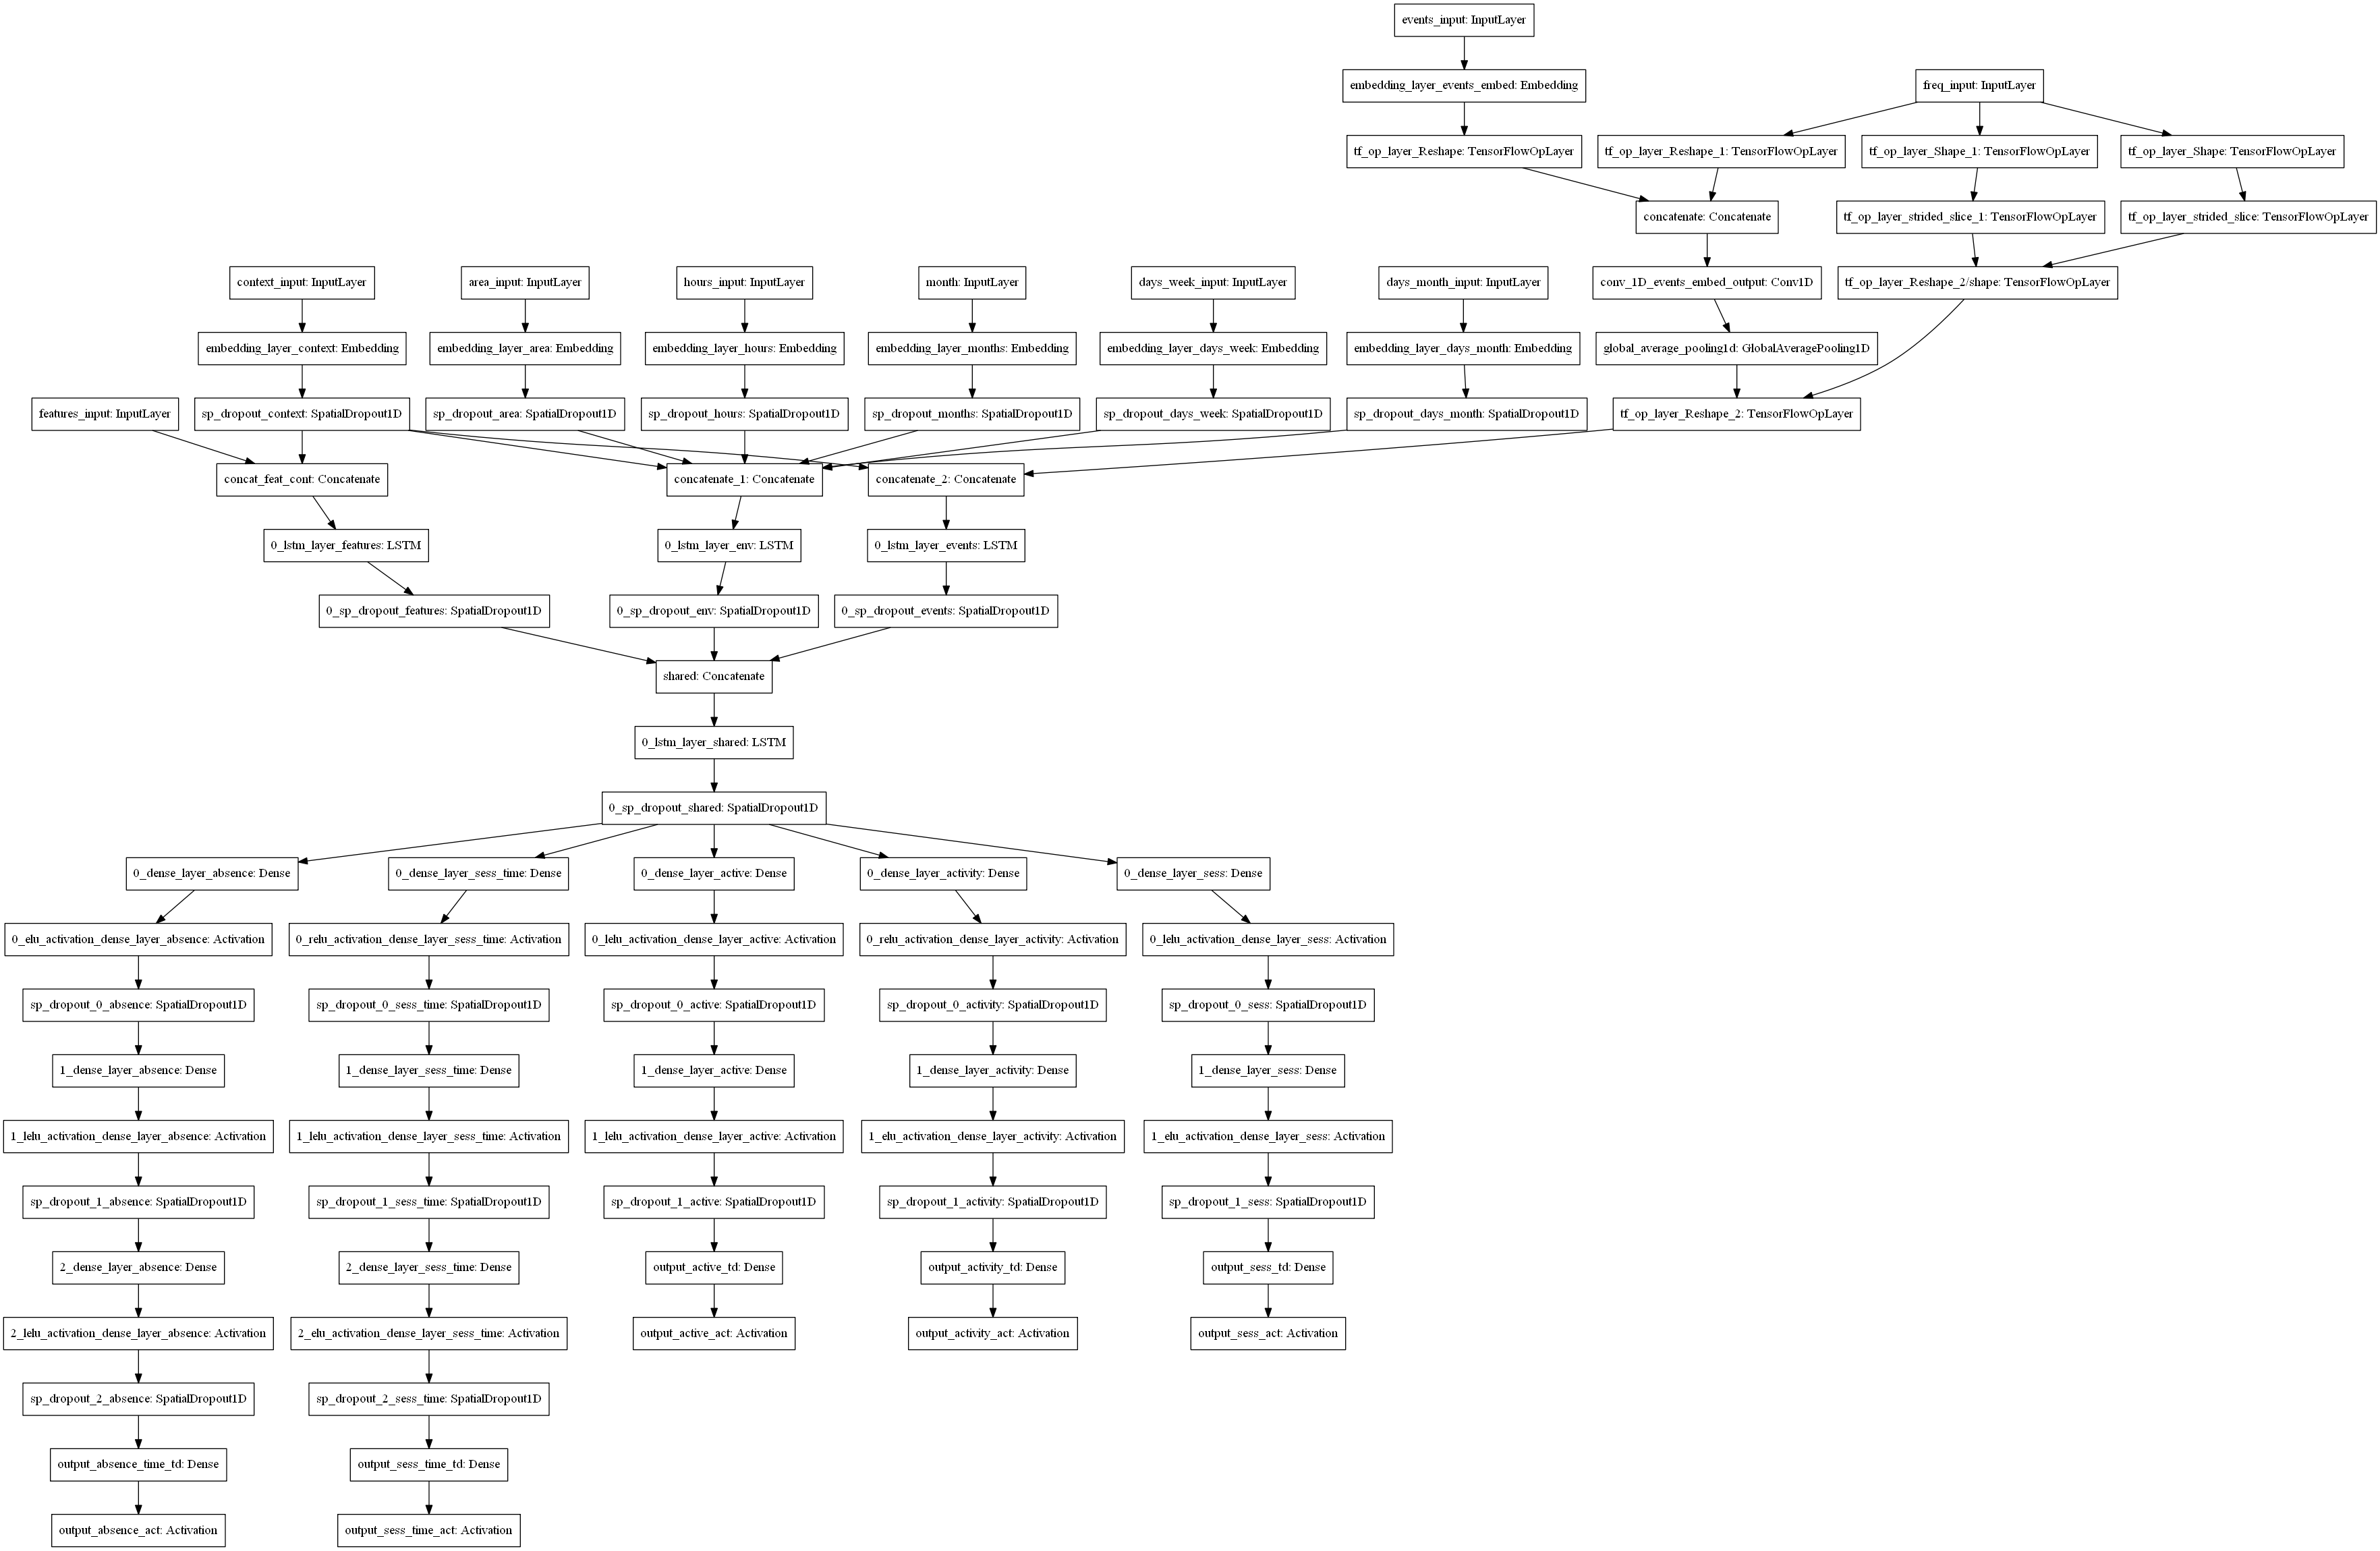
\includegraphics[width=\textwidth,height=0.7\textheight,keepaspectratio]{images/appendix_B/rnn_env_even_3.png}
\caption[\textbf{RNN Environment-Events DAG - Section \ref{model_architecture_3}}]{Directed acyclic graph representation of the RNN Environment-Events architecture proposed in section \ref{model_architecture_3}}
\label{rnn_env_even_dag}
\end{figure}